% Options for packages loaded elsewhere
\PassOptionsToPackage{unicode}{hyperref}
\PassOptionsToPackage{hyphens}{url}
\documentclass[
]{article}
\usepackage{xcolor}
\usepackage[margin=1in]{geometry}
\usepackage{amsmath,amssymb}
\setcounter{secnumdepth}{5}
\usepackage{iftex}
\ifPDFTeX
  \usepackage[T1]{fontenc}
  \usepackage[utf8]{inputenc}
  \usepackage{textcomp} % provide euro and other symbols
\else % if luatex or xetex
  \usepackage{unicode-math} % this also loads fontspec
  \defaultfontfeatures{Scale=MatchLowercase}
  \defaultfontfeatures[\rmfamily]{Ligatures=TeX,Scale=1}
\fi
\usepackage{lmodern}
\ifPDFTeX\else
  % xetex/luatex font selection
\fi
% Use upquote if available, for straight quotes in verbatim environments
\IfFileExists{upquote.sty}{\usepackage{upquote}}{}
\IfFileExists{microtype.sty}{% use microtype if available
  \usepackage[]{microtype}
  \UseMicrotypeSet[protrusion]{basicmath} % disable protrusion for tt fonts
}{}
\makeatletter
\@ifundefined{KOMAClassName}{% if non-KOMA class
  \IfFileExists{parskip.sty}{%
    \usepackage{parskip}
  }{% else
    \setlength{\parindent}{0pt}
    \setlength{\parskip}{6pt plus 2pt minus 1pt}}
}{% if KOMA class
  \KOMAoptions{parskip=half}}
\makeatother
\usepackage{longtable,booktabs,array}
\usepackage{calc} % for calculating minipage widths
% Correct order of tables after \paragraph or \subparagraph
\usepackage{etoolbox}
\makeatletter
\patchcmd\longtable{\par}{\if@noskipsec\mbox{}\fi\par}{}{}
\makeatother
% Allow footnotes in longtable head/foot
\IfFileExists{footnotehyper.sty}{\usepackage{footnotehyper}}{\usepackage{footnote}}
\makesavenoteenv{longtable}
\usepackage{graphicx}
\makeatletter
\newsavebox\pandoc@box
\newcommand*\pandocbounded[1]{% scales image to fit in text height/width
  \sbox\pandoc@box{#1}%
  \Gscale@div\@tempa{\textheight}{\dimexpr\ht\pandoc@box+\dp\pandoc@box\relax}%
  \Gscale@div\@tempb{\linewidth}{\wd\pandoc@box}%
  \ifdim\@tempb\p@<\@tempa\p@\let\@tempa\@tempb\fi% select the smaller of both
  \ifdim\@tempa\p@<\p@\scalebox{\@tempa}{\usebox\pandoc@box}%
  \else\usebox{\pandoc@box}%
  \fi%
}
% Set default figure placement to htbp
\def\fps@figure{htbp}
\makeatother
% definitions for citeproc citations
\NewDocumentCommand\citeproctext{}{}
\NewDocumentCommand\citeproc{mm}{%
  \begingroup\def\citeproctext{#2}\cite{#1}\endgroup}
\makeatletter
 % allow citations to break across lines
 \let\@cite@ofmt\@firstofone
 % avoid brackets around text for \cite:
 \def\@biblabel#1{}
 \def\@cite#1#2{{#1\if@tempswa , #2\fi}}
\makeatother
\newlength{\cslhangindent}
\setlength{\cslhangindent}{1.5em}
\newlength{\csllabelwidth}
\setlength{\csllabelwidth}{3em}
\newenvironment{CSLReferences}[2] % #1 hanging-indent, #2 entry-spacing
 {\begin{list}{}{%
  \setlength{\itemindent}{0pt}
  \setlength{\leftmargin}{0pt}
  \setlength{\parsep}{0pt}
  % turn on hanging indent if param 1 is 1
  \ifodd #1
   \setlength{\leftmargin}{\cslhangindent}
   \setlength{\itemindent}{-1\cslhangindent}
  \fi
  % set entry spacing
  \setlength{\itemsep}{#2\baselineskip}}}
 {\end{list}}
\usepackage{calc}
\newcommand{\CSLBlock}[1]{\hfill\break\parbox[t]{\linewidth}{\strut\ignorespaces#1\strut}}
\newcommand{\CSLLeftMargin}[1]{\parbox[t]{\csllabelwidth}{\strut#1\strut}}
\newcommand{\CSLRightInline}[1]{\parbox[t]{\linewidth - \csllabelwidth}{\strut#1\strut}}
\newcommand{\CSLIndent}[1]{\hspace{\cslhangindent}#1}
\setlength{\emergencystretch}{3em} % prevent overfull lines
\providecommand{\tightlist}{%
  \setlength{\itemsep}{0pt}\setlength{\parskip}{0pt}}
\usepackage{bookmark}
\IfFileExists{xurl.sty}{\usepackage{xurl}}{} % add URL line breaks if available
\urlstyle{same}
\hypersetup{
  pdftitle={CARTEpigenoQC: A Quality Control Toolkit for CAR-T Single-Cell Epigenomic Data},
  pdfauthor={Kaitao Lai1},
  hidelinks,
  pdfcreator={LaTeX via pandoc}}

\title{CARTEpigenoQC: A Quality Control Toolkit for CAR-T Single-Cell
Epigenomic Data}
\author{Kaitao Lai\textsuperscript{1}}
\date{2025-07-28}

\begin{document}
\maketitle

\textsuperscript{1} University of Sydney

\section{Summary}\label{summary}

CARTEpigenoQC is an R-based toolkit designed to streamline quality
control (QC) for single-cell epigenomic datasets involving Chimeric
Antigen Receptor (CAR)-engineered T cells. With the growing application
of scATAC-seq, scCUT\&Tag, and scBS-seq to characterize CAR-T cell
states (Satpathy et al. 2019), it has become critical to perform
customized QC that not only addresses standard metrics like FRiP
(Fraction of Reads in Peaks) and TSS enrichment, but also directly
detects signal from CAR vector insertion sites.

CARTEpigenoQC supports both 10x Genomics and non-10x data formats and
produces HTML and PNG summary outputs suited for exploratory analysis
and regulatory-grade preclinical reporting. It is intended to assist
researchers, core facilities, and translational immunologists in
ensuring the validity of single-cell epigenomic profiling of engineered
T cells (Finck and al. 2022; Robinson, Nguyen, and Sadelain 2023).

\section{Statement of Need}\label{statement-of-need}

Despite the rise in single-cell chromatin profiling technologies in
immunotherapy, current QC pipelines do not provide functionality to
assess CAR vector integration in scATAC-seq or related datasets.
Existing tools like ArchR (Granja et al. 2021), Signac (Stuart et al.
2021), or SnapATAC (Fang et al. 2021) focus on general chromatin metrics
but lack transgene-specific support. CARTEpigenoQC fills this gap by
integrating standard QC (e.g., FRiP, duplication, peak overlap) with
direct inspection of vector signal such as \(\text{EF1-}\alpha\), PGK1,
or TRAC locus insertions that are common in CAR constructs (Eyquem et
al. 2017).

This tool was inspired by the increasing use of vector-based gene
therapies and the demand for preclinical quality pipelines (Maude et al.
2018). It is lightweight, fast, and does not require complex
dependencies. It generates clean, reproducible Markdown-based reports
suitable for clinical handoff, regulatory review, or publication.

\section{Features}\label{features}

\begin{itemize}
\tightlist
\item
  FRiP calculation per cell using fragment overlaps with peak regions.
\item
  Visualization of CAR vector site coverage across single cells.
\item
  Markdown-based report with interactive and static plots.
\item
  Compatible with 10x Genomics `fragments.tsv.gz', ArchR fragments, and
  BED-formatted CAR insertion sites.
\item
  Designed for reproducibility and integration into preclinical
  immunotherapy pipelines.
\end{itemize}

\section{Example Usage}\label{example-usage}

CARTEpigenoQC includes a `run\_qc.R' script and report template. When
supplied with fragment files and a BED file of CAR insertion
coordinates, it calculates QC metrics and generates a self-contained
HTML report.

\section{Example Outputs}\label{example-outputs}

\subsection{FRiP Score Distribution}\label{frip-score-distribution}

This histogram visualizes the distribution of FRiP (Fraction of Reads in
Peaks) across all cells. A peak around 0.2--0.4 is expected for
high-quality scATAC-seq data (Chen et al. 2019). A right-skewed
distribution is typical, and cells with FRiP \textless{} 0.2 may be
filtered out in downstream analyses.

\begin{figure}
\centering
\pandocbounded{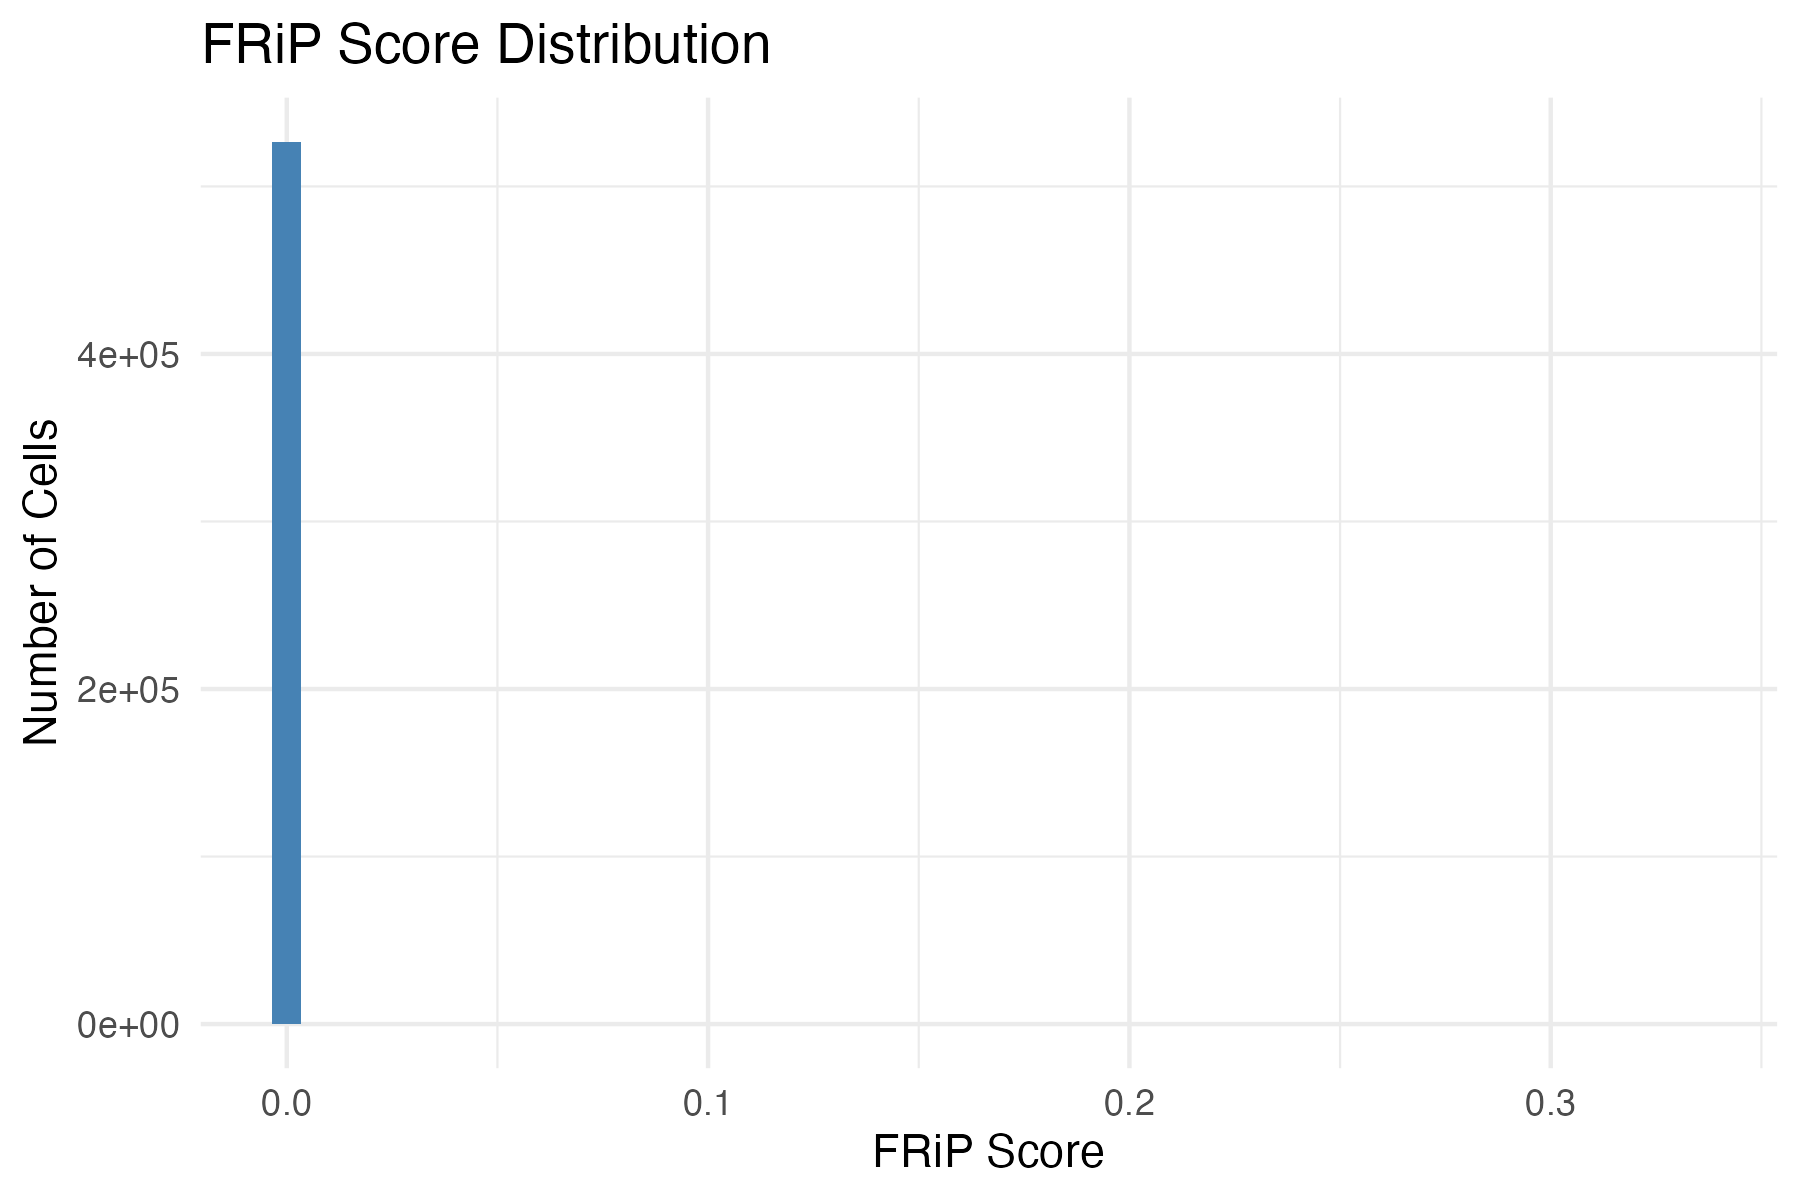
\includegraphics[keepaspectratio,alt={FRiP Histogram: Distribution of FRiP (Fraction of Reads in Peaks) scores across all single cells. This histogram visualizes the signal enrichment, with higher FRiP values indicating better signal-to-noise ratios and higher data quality in single-cell chromatin profiling.}]{figures/example_frip_plot.png}}
\caption{FRiP Histogram: Distribution of FRiP (Fraction of Reads in
Peaks) scores across all single cells. This histogram visualizes the
signal enrichment, with higher FRiP values indicating better
signal-to-noise ratios and higher data quality in single-cell chromatin
profiling.}
\end{figure}

\subsection{Top Cells by FRiP}\label{top-cells-by-frip}

This table lists the top 20 cells with the highest FRiP scores. These
cells often exhibit clearer chromatin signatures and are more
informative for downstream applications like motif enrichment or
regulatory network analysis.

\subsection{Top FRiP Table}\label{top-frip-table}

\begingroup
\small  % can also try \footnotesize, \scriptsize, or \tiny

\begin{longtable}[]{@{}
  >{\raggedright\arraybackslash}p{(\linewidth - 8\tabcolsep) * \real{0.0597}}
  >{\raggedright\arraybackslash}p{(\linewidth - 8\tabcolsep) * \real{0.3582}}
  >{\raggedright\arraybackslash}p{(\linewidth - 8\tabcolsep) * \real{0.1194}}
  >{\raggedright\arraybackslash}p{(\linewidth - 8\tabcolsep) * \real{0.1642}}
  >{\raggedright\arraybackslash}p{(\linewidth - 8\tabcolsep) * \real{0.2985}}@{}}
\toprule\noalign{}
\begin{minipage}[b]{\linewidth}\raggedright
\#
\end{minipage} & \begin{minipage}[b]{\linewidth}\raggedright
Barcode
\end{minipage} & \begin{minipage}[b]{\linewidth}\raggedright
Total
\end{minipage} & \begin{minipage}[b]{\linewidth}\raggedright
In Peaks
\end{minipage} & \begin{minipage}[b]{\linewidth}\raggedright
FRiP
\end{minipage} \\
\midrule\noalign{}
\endhead
\bottomrule\noalign{}
\endlastfoot
1 & ACAGAAACAGGTCTGC-1 & 3 & 1 & 0.333333333333333 \\
2 & ACTGTCCCATAGACGG-1 & 6 & 1 & 0.166666666666667 \\
3 & GCAGCTGTCAATTGGC-1 & 17 & 1 & 0.058823529411765 \\
4 & TTGTCTAAGCAGTAGC-1 & 24 & 1 & 0.041666666666667 \\
5 & AGTTACGGTATCTGCA-1 & 1457 & 2 & 0.001372683596431 \\
6 & CAGTATGAGTCGTATC-1 & 781 & 1 & 0.001280409731114 \\
7 & ACTATTCTCGGATAAA-1 & 1695 & 2 & 0.001179941002950 \\
8 & TCAGTCCGTGGACGAT-1 & 957 & 1 & 0.001044932079415 \\
9 & AATGCCAGTGGCCTCA-1 & 966 & 1 & 0.001035196687371 \\
10 & AATGGCTGTCCCTTTG-1 & 1002 & 1 & 0.000998003992016 \\
11 & GCAGATTAGCCCATGC-1 & 1009 & 1 & 0.000991080277502 \\
12 & AGTCAACAGGCGTCCT-1 & 1020 & 1 & 0.000980392156863 \\
13 & TGCCTGTTCGCAGATT-1 & 1021 & 1 & 0.000979431929481 \\
14 & CCCTCTCTCTTAACGG-1 & 1059 & 1 & 0.000944287063267 \\
15 & CACATGACATATTGGC-1 & 1064 & 1 & 0.000939849624060 \\
16 & CGCTATCTCGCTCTAC-1 & 1094 & 1 & 0.000914076782450 \\
17 & TTAACGGAGTCGATAA-1 & 2228 & 2 & 0.000897666068223 \\
18 & GAAGAGCCAAAGCATA-1 & 1208 & 1 & 0.000827814569536 \\
19 & CCCGTTAAGGCAATTA-1 & 1234 & 1 & 0.000810372771475 \\
20 & CAACGTAGTAAGTCTC-1 & 1243 & 1 & 0.000804505229284 \\
\end{longtable}

\endgroup

Table 1: Top FRiP: Top 20 barcodes ranked by FRiP (Fraction of Reads in
Peaks) scores. This table summarizes the total number of reads, number
of reads overlapping peaks, and calculated FRiP values for each cell
barcode, providing an indicator of signal-to-noise ratio in single-cell
epigenomic data.

\subsection{CAR Insertion Site Coverage
Heatmap}\label{car-insertion-site-coverage-heatmap}

The heatmap shows per-cell read coverage across CAR vector insertion
sites (e.g., EF1a, PGK1, TRAC). Each row represents a cell barcode, and
each column represents a CAR target site. This allows visualization of
which cells are likely to carry vector insertions and where signal
enrichment occurs, helping to verify construct delivery or identify
mosaicism in editing (Torres et al. 2022).

\begin{figure}
\centering
\pandocbounded{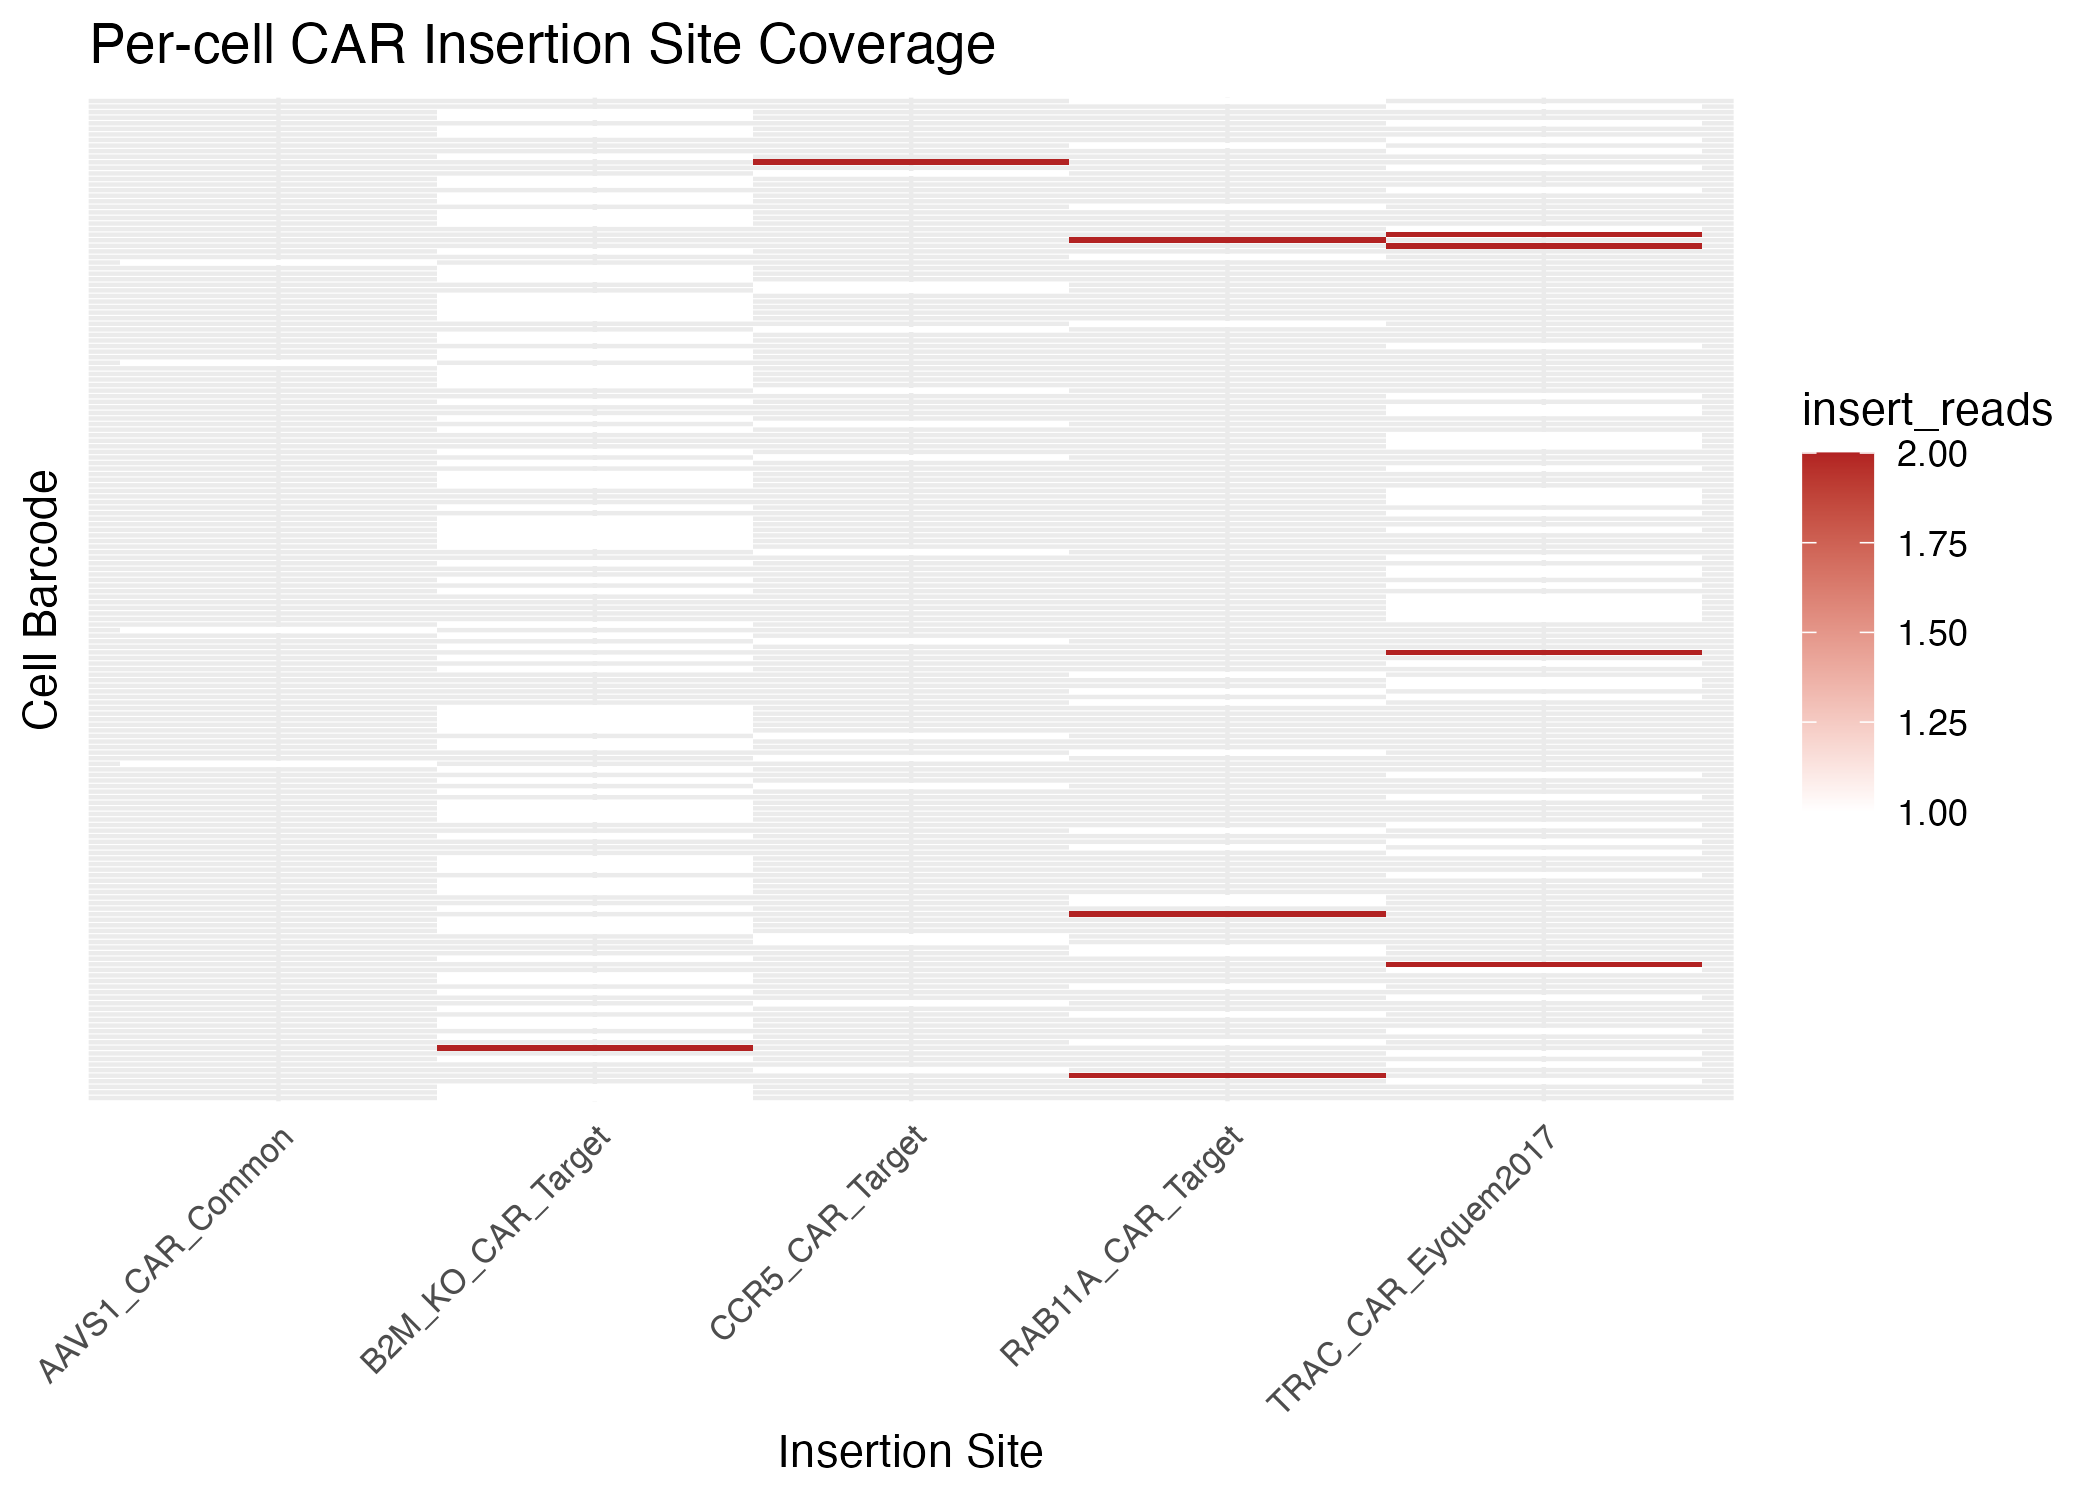
\includegraphics[keepaspectratio,alt={CAR Insertion Heatmap: Heatmap showing CAR (Chimeric Antigen Receptor) insertion site coverage across individual cells. Each row corresponds to a target site, and each column represents a single cell, with color intensity indicating the number of reads supporting integration. This highlights the distribution and specificity of CAR insertions in the dataset.}]{figures/car_coverage_heatmap.png}}
\caption{CAR Insertion Heatmap: Heatmap showing CAR (Chimeric Antigen
Receptor) insertion site coverage across individual cells. Each row
corresponds to a target site, and each column represents a single cell,
with color intensity indicating the number of reads supporting
integration. This highlights the distribution and specificity of CAR
insertions in the dataset.}
\end{figure}

\subsection{Top CAR Sites by Total
Coverage}\label{top-car-sites-by-total-coverage}

This table summarizes the top 10 CAR insertion sites ranked by the total
number of reads mapped to each site across all cells. It helps identify
the most active or consistently covered transgene targets, which is
critical in validating vector design and insertion stability (Frangieh
et al. 2021).

\section{Top CAR Insertion Site Read
Counts}\label{top-car-insertion-site-read-counts}

\begingroup
\small  % can also try \footnotesize, \scriptsize, or \tiny

\begin{longtable}[]{@{}ll@{}}
\toprule\noalign{}
Site & Total Reads \\
\midrule\noalign{}
\endhead
\bottomrule\noalign{}
\endlastfoot
B2M\_KO\_CAR\_Target & 91 \\
TRAC\_CAR\_Eyquem2017 & 53 \\
RAB11A\_CAR\_Target & 24 \\
CCR5\_CAR\_Target & 18 \\
AAVS1\_CAR\_Common & 4 \\
\end{longtable}

\endgroup

Table 2: Top CAR Insertion Site Read Counts: Read counts mapped to the
top CAR (Chimeric Antigen Receptor) insertion sites. Each row represents
a genomic target site with the corresponding number of supporting reads,
indicating the relative abundance of CAR integrations across different
loci.

\section{Repository and Installation}\label{repository-and-installation}

The source code is hosted on GitHub:\\
\url{https://github.com/biosciences/CARTEpigenoQC}

\section{Acknowledgements}\label{acknowledgements}

The author thanks collaborators at the University of Sydney for insights
into CAR-T clinical pipelines, and for pipeline development guidance.

\section*{References}\label{references}
\addcontentsline{toc}{section}{References}

\protect\phantomsection\label{refs}
\begin{CSLReferences}{1}{0}
\bibitem[\citeproctext]{ref-chen2019}
Chen, Hanqing, Caleb A Lareau, Thomas Andreani, Matthew E Vinyard,
Sandra P Garcia, Kyle Clement, Miguel A Andrade-Navarro, and Jason D
Buenrostro. 2019. {``High-Throughput Sequencing of the Transcriptome and
Epigenome of Single Cells.''} \emph{Nature Reviews Genetics} 20 (10):
631--47.

\bibitem[\citeproctext]{ref-eyquem2017}
Eyquem, Julien, Jorge Mansilla-Soto, Theodoros Giavridis, Stefan JC van
der Stegen, Mohamad Hamieh, Kristen M Cunanan, Alexander Odak, Mehmet
Gonen, and Michel Sadelain. 2017. {``Targeting a CAR to the TRAC Locus
with CRISPR/Cas9 Enhances Tumour Rejection.''} \emph{Nature} 543 (7643):
113--17.

\bibitem[\citeproctext]{ref-fang2021}
Fang, Rui, Sebastian Preissl, Yanxiao Li, Xinyi Hou, Julian Lucero,
Xinyi Wang, Amir Motamedi, et al. 2021. {``SnapATAC: A Comprehensive
Analysis Package for Single Cell ATAC-Seq.''} \emph{bioRxiv}.
\url{https://doi.org/10.1101/615179}.

\bibitem[\citeproctext]{ref-finck2022}
Finck, Alexander, and et al. 2022. {``Epigenetic and Transcriptional
Profiling of CAR t Cells Reveals Insights into t Cell Exhaustion and
Persistence.''} \emph{Nature Medicine} 28 (3): 467--79.

\bibitem[\citeproctext]{ref-frangieh2021}
Frangieh, Cyrus J, John C Melms, Pratik I Thakore, and et al. 2021.
{``Multimodal Pooled Perturb-Seq Reveals Synergistic and Antagonistic
Gene Modules in the Immune Response.''} \emph{Cell} 184 (3):
882--895.e21.

\bibitem[\citeproctext]{ref-granja2021}
Granja, Jeffrey M, M Ryan Corces, Sarah E Pierce, Seyed T Bagdatli,
Harinder Choudhry, Howard Y Chang, and William J Greenleaf. 2021.
{``ArchR Is a Scalable Software Package for Integrative Single-Cell
Chromatin Accessibility Analysis.''} \emph{Nature Genetics} 53 (3):
403--11.

\bibitem[\citeproctext]{ref-maude2018}
Maude, Shannon L, Theodore W Laetsch, Jochen Buechner, Silvia Rives,
Michel Boyer, Henri Bittencourt, Peter Bader, et al. 2018.
{``Tisagenlecleucel in Children and Young Adults with b-Cell
Lymphoblastic Leukemia.''} \emph{New England Journal of Medicine} 378
(5): 439--48.

\bibitem[\citeproctext]{ref-robinson2023}
Robinson, Kimberly, Mai Nguyen, and Michel Sadelain. 2023.
{``Single-Cell Epigenomic Profiling in Immunotherapy: New Tools and
Perspectives.''} \emph{Trends in Immunology} 44 (2): 115--29.

\bibitem[\citeproctext]{ref-satpathy2019}
Satpathy, Ansuman T, Jeffrey M Granja, Kathryn E Yost, Yuhan Qi,
Francesco Meschi, Gavin P McDermott, Ben N Olsen, et al. 2019.
{``Massively Parallel Single-Cell Chromatin Landscapes of Human Immune
Cell Development and Intratumoral t Cell Exhaustion.''} \emph{Nature
Biotechnology} 37 (8): 925--36.

\bibitem[\citeproctext]{ref-stuart2021}
Stuart, Tim, Avi Srivastava, Shila Madad, Caleb A Lareau, and Rahul
Satija. 2021. {``Signac: Multimodal Single-Cell Chromatin Analysis with
r.''} \emph{bioRxiv}. \url{https://doi.org/10.1101/2020.11.09.373613}.

\bibitem[\citeproctext]{ref-torres2022}
Torres, David, Ankit Tiwari, Jinyu Du, et al. 2022. {``Comprehensive
Single-Cell CRISPR Screening Reveals a Novel Vector Integration Bias in
t Cells.''} \emph{Nature Biotechnology} 40: 1636--45.

\end{CSLReferences}

\end{document}
